\section{Grundvand}

\begin{frame}{Kvælstofforurening af grundvand}
  \textbf{Nitatkoncentrationer i grundvand og drikkevand:}
  \begin{itemize}
    \item Skal være under 50 mg/l for at undgå sundhedsfare og eutrofiering ved udstrømning til overfladevand.
    \begin{itemize}
      \item[$\rightarrow$] \normalsize Grundvandsboringer \textit{under (over)} kravværdien siges at have \textit{god (dårlig)} kemisk tilstand.
    \end{itemize}
    \item Vi benytter imputering og tildeler samme vægt til alle boringer, der indgår i Grundvandsovervågningen (GRUMO).
  \end{itemize}
  \vfill
\end{frame}

\begin{frame}{Kvælstofforurening af grundvand}
  \center
  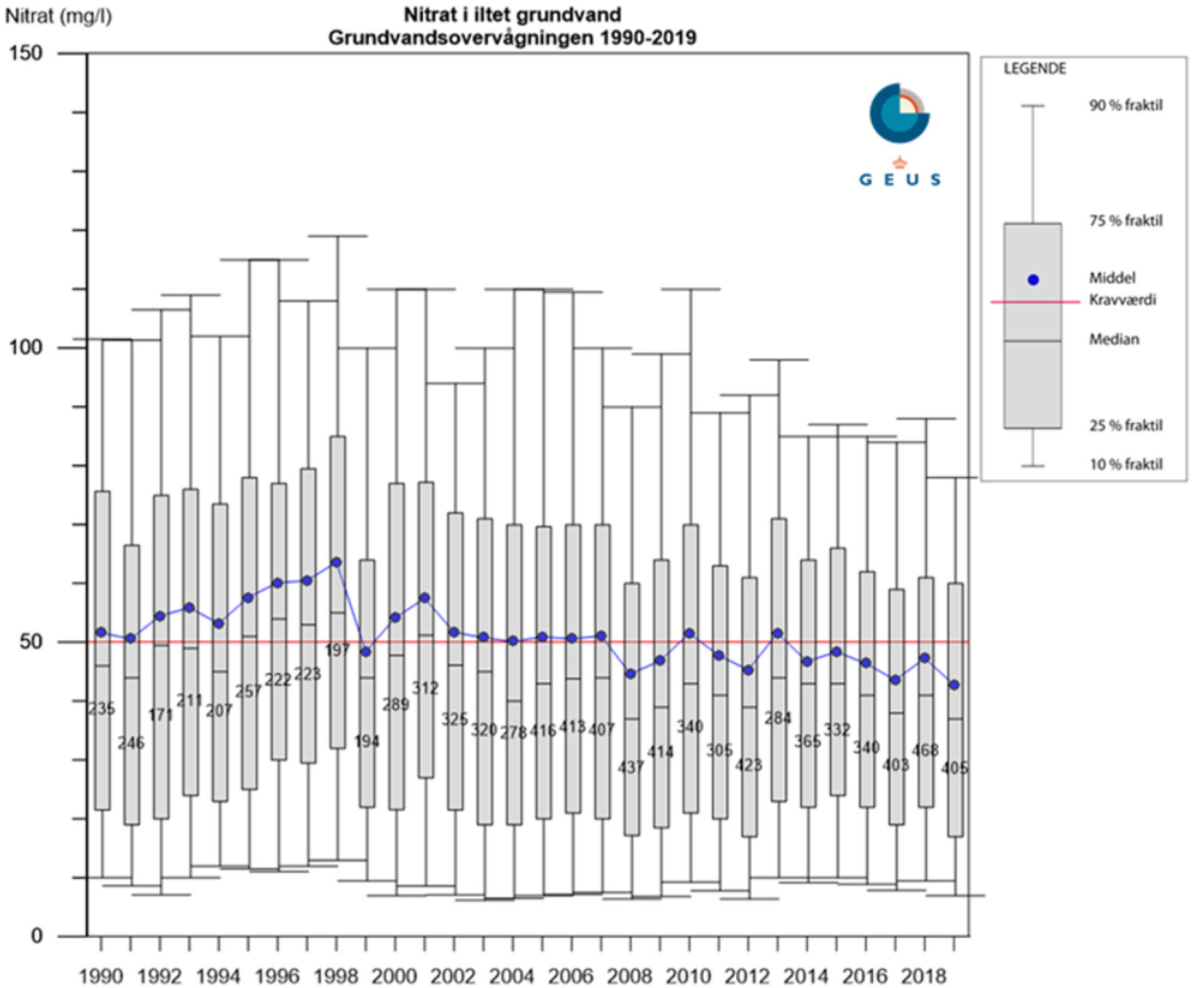
\includegraphics[width=.8\textwidth]{figures/nitrate}
\end{frame}

\begin{frame}{Pesticider i grundvand}
    \textbf{Det er meget omskifteligt, hvilke pesticider der anvendes og hvilke anses for at være sundhedsskadelige:}
    \begin{itemize}
      \item Nye analysemetoder udvikles og tages i anvendelse løbende.
      \item Derfor er det umuligt at konstruere en langvarig tidsserie for den samlede pesticidkoncentration, som er det mindste retvisende.
    \end{itemize}
    \textit{\textbf{Vi begrænser derfor vores analyse af grundvandet til nitrat.}}
\end{frame}

\begin{frame}{Enkelte pesticider i grundvand (1998-2018)}
  \center
  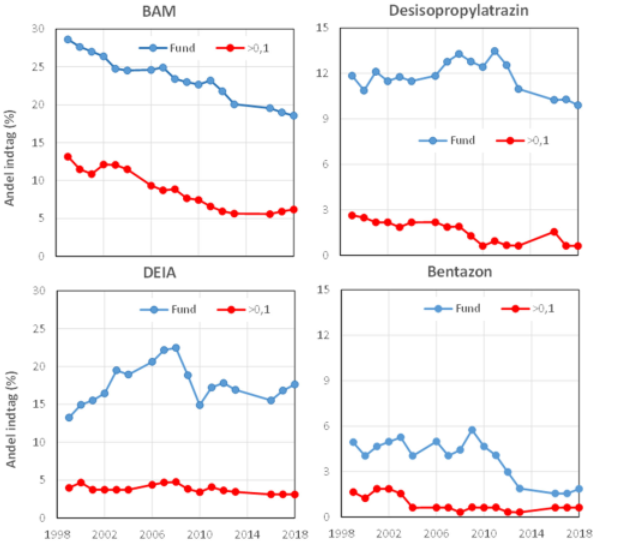
\includegraphics[width=.75\textwidth]{figures/pesticides}
\end{frame}

